%
% Annual Cognitive Science Conference
% Sample LaTeX Paper -- Proceedings Format
%

% Original : Ashwin Ram (ashwin@cc.gatech.edu)       04/01/1994
% Modified : Johanna Moore (jmoore@cs.pitt.edu)      03/17/1995
% Modified : David Noelle (noelle@ucsd.edu)          03/15/1996
% Modified : Pat Langley (langley@cs.stanford.edu)   01/26/1997
% Latex2e corrections by Ramin Charles Nakisa        01/28/1997
% Modified : Tina Eliassi-Rad (eliassi@cs.wisc.edu)  01/31/1998
% Modified : Trisha Yannuzzi (trisha@ircs.upenn.edu) 12/28/1999 (in process)
% Modified : Mary Ellen Foster (M.E.Foster@ed.ac.uk) 12/11/2000
% Modified : Ken Forbus                              01/23/2004
% Modified : Eli M. Silk (esilk@pitt.edu)            05/24/2005
% Modified : Niels Taatgen (taatgen@cmu.edu)         10/24/2006
% Modified : David Noelle (dnoelle@ucmerced.edu)     11/19/2014

%% Change "letterpaper" in the following line to "a4paper" if you must.

\documentclass[10pt,letterpaper]{article}

\usepackage{cogsci}
\usepackage{pslatex}
\usepackage{apacite}
\usepackage{graphicx}
\usepackage{subcaption}
\usepackage{natbib}

% New command: footnote without reference
\newcommand\blfootnote[1]{%
  \begingroup
  \renewcommand\thefootnote{}\footnote{#1}%
  \addtocounter{footnote}{-1}%
  \endgroup
}


\title{Learning Inductive Biases with Developmentally-informed Neural Networks}
%\title{CogSci 2018 Paper (Title TBD)}

\author{{\large \bf Reuben Feinman (reuben.feinman@nyu.edu)} \\
  Center for Neural Science \\
  New York University
  \AND {\large \bf Brenden M. Lake (brenden@nyu.edu)} \\
  Department of Psychology and Center for Data Science \\
  New York University}


\begin{document}

\maketitle


\begin{abstract}
    People use rich prior knowledge about the world in order
to efficiently learn new concepts. These priors--commonly referred to as
``inductive biases"--pertain to the space of internal models considered by a
learner, and they help maximize the amount of information that is extracted
from limited data. Recently, it was shown that performance-optimized
deep neural networks (DNNs) develop inductive biases similar to those
possessed by human children. However, these models use unrealistic training
data, and it remains unclear whether they develop their biases in the same way
as humans. We investigate the development and influence of inductive biases
in DNNs using an experimental paradigm borrowed from develpmental psychology.
We find that simple neural network models can develop inductive
biases from as few as 2 examples of each concept, and that these biases tend
to grow with depth in the network. The development of these biases predicts
the onset of vocabulary acceleration in our networks, a finding that mimicks
human children.

\textbf{Keywords:}
learning-to-learn; neural networks; inductive biases
\end{abstract}

\section{Introduction}

Humans possess the remarkable ability to learn a new concept from seeing just a
few examples. A child who is learning her first few words can easily pick up
the meaning of the word ``fork" after observing only one or a handful of forks
\citep{Bloom2000}. In contrast, state-of-the-art artificial learning systems use
hundreds or thousands of examples when learning to recognize the same objects
\citep[e.g.,][]{Krizhevsky2012, Szegedy2015}. Consequently, significant
effort is ongoing to understand what neural and cognitive mechanisms enable
efficient concept learning \citep{Lake2017}. In this paper, we perform a series
of developmentally-informed neural network experiments to study the
computational basis of efficient word learning. \footnote{All experiments can be
reproduced using the code repository located at
\url{http://github.com/rfeinman/learning-to-learn}.}

\begin{figure}[h!]
    \begin{center}
        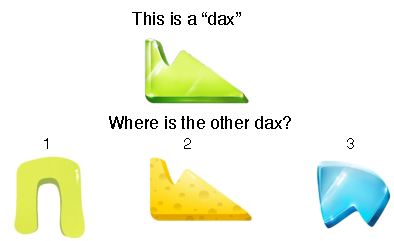
\includegraphics[width=0.35\textwidth]{figures/shape_bias_demo.pdf}
    \end{center}
    \caption{The shape bias. Children learn that objects with the same name
    tend to have the same shape, and thus option 2 above is likely the right
    answer. This inductive bias helps with future word learning.}
    \label{fig:shape_bias_demo}
\end{figure}

If humans extrapolate beyond the presented data, then another source of
information must make up the difference; prior background knowledge must
delimit the hypothesis space during learning \citep{Tenenbaum2011, Lake2017}. By
constraining the space of models considered by the learner, these priors,
referred to herein as ``inductive biases," help the learner make inferences
that go far beyond the observed data. As one manifestation, human children make
use of the shape bias--the assumption that objects that have the same name will
tend to have the same shape--when learning new object names, and thus shape is
more important than color, material and other properties when generalizing a
new label to new examples (Fig. \ref{fig:shape_bias_demo}) \citep{Landau1988}.
Similarly, children assume that object names are mutually exclusive, i.e. that
a novel name probably refers to a novel object rather than a familiar object
\citep{Markman1988}. Although the origin of inductive biases is not always
clear, results show that children, adults and primates can ``learn-to-learn" or
form higher-order generalizations that can improve the efficiency of future
learning \citep{Harlow1949, Smith2002, Dewar2010}.

Cognitive scientists have proposed a number of computational models to explain
how inductive biases are acquired and harnessed for future learning.
Hierarchical Bayesian Models (HBMs) enable probabilistic inference at multiple
levels simultaneously, allowing the model to learn the structure of individual
concepts while simultaneously learning about the structure of concepts in
general (i.e., learning a prior on new concepts)
\citep{Gelman2013, Kemp2007, Salakhutdinov2012}. These models have been used to
explain various forms of ``learning-to-learn" including learning a shape bias
\citep{Kemp2007}, yet it is currently difficult to apply HBMs to the type of
raw, high-dimensional sensory data that children receive, such as images or
audio waves. In some cases, HBMs and related approaches have been applied
successfully to raw high-dimensional data such as when learning handwritten
characters \citep{Lake2015}, but with the help of domain-specific knowledge and
engineering. In contrast, recent progress in training deep neural networks
shows how relatively generic architectures can learn effectively from raw data
\citep{LeCun2015}, providing the potential bridge between controlled simulations
with synthetic data \citep[e.g.,][]{Colunga2005} and large-scale real-world
object recognition tasks with raw data \citep[e.g.,][]{Ritter2017}. Here, we
take advantage of this connection by using neural networks to study
learning-to-learn in several different settings of varying stimulus complexity,
with the goal of isolating the fundamentals of the learning dynamics.

Most related to our work here are studies by \cite{Colunga2005} and
\cite{Ritter2017} investigating neural network accounts of shape bias
development. \cite{Colunga2005} showed that a simple neural network model,
trained via Hebbian learning, can acquire the shape bias when presented with
datasets comparable to human developmental studies. However, these simulations
operate on highly simplified bit-vector data, and it is unclear how their
results generalize to more realistic stimuli. Furthermore, the authors did not
systematically vary the structure of the training set, so we do not know the
exact conditions in which biases arise, nor whether current models are
sufficient to explain it. In a recent study, building on recent advances in
object recognition, \cite{Ritter2017} found that performance-optimized deep
neural networks (DNNs) develop the shape bias over the course of learning when
trained on the popular ImageNet classification dataset consisting of raw
naturalistic images. Although these results highlight an exciting possible
connection between DNNs and developmental psychology, many questions remain.
ImageNet--which contains thousands of labeled examples of each visual
concept--is a poor proxy for human developmental learning sets. Whether or not
these models can acquire the same bias with a training set comparable to humans
remains unknown; an answer to this question may help to explain the
developmental process in children. Furthermore, while the development of the
shape bias is known to predict the onset of vocabulary acceleration in children
\citep{GershkoffStowe2004}, we do not know whether the same holds for DNNs.

We investigate the development and influence of inductive biases in neural
network models using artificial object stimuli designed to closely mimic
developmental studies with human children. Borrowing the experimental paradigm
of \cite{Smith2002}, we evaluate the first- and second-order generalization
capabilities of neural networks trained with variable-sized datasets. Beginning
with simple bit-vector data akin to \cite{Colunga2005}, we systematically vary
the number of categories and the number of exemplars in the training set,
recording generalization performance at each pairing. Parallel experiments are
then performed with RGB image data, where each image consists of a 2D object
with a particular shape, color and texture that is shifted and placed over
white background. For each the bit-vector and RGB image data, we investigate
the parametric relationship between bias strength and attribute similarity in
our models by systematically varying the shape, color and texture attributes of
select test stimuli. Similarly, we evaluate bias strength as a function of
depth in the network. In a final set of experiments, we investigate the
correlation between shape bias acquisition and the rate of concept learning in
our networks, mirroring an analogous study from human developmental psychology
\citep{GershkoffStowe2004}.




\section{Experimental Paradigm}
\label{sec:experimental_paradigm}
We first set out to model the infant learning tasks described in
\citet{Smith2002} using simple neural networks. In order to do so, we use
artificial toy data that is designed to mimic the training data described in
the paper. Each object sample is assigned a shape, texture and color value.
There are two types of model evaluations performed, both drawn from
\cite{Smith2002}.

{\bf1. First-order generalization test}: For the first-order generalization
test, infants are asked to evaluate novel instances of familiar objects. To
simulate this test, we train our neural network models to classify objects,
ensuring that objects of the same category are assigned the same shape. Then,
we build a test set by creating one novel exemplar of each category that
appeared in the training set. The novel exemplar has the same shape as the
training exemplars of that category, but a new color and texture combination.
Accuracy is defined as the fraction of test images that are correctly
classified by the model. This test is repeated for different training set
sizes, i.e. different combinations of \{\textit{\# categories},
\textit{\# exemplars}\}. It is important to note that as \textit{\# categories}
increases, the first-order task becomes more difficult.

{\bf2. Second-order generalization test}: For the second-order generalization
test, infants are presented with an exemplar of a novel object category as a
baseline. Then, they are shown 3 comparison objects: one which has the same
shape as the baseline, one with the same color, and one with the same texture.
In each case, the other 2 features are different from the baseline. The infants
are asked to select which of the 3 comparison objects are of the same category
as the baseline object. We simulate this test by creating an evaluation set
containing groupings of 4 samples: the baseline, the shape constant, the color
constant, and the texture constant. Each grouping serves as one test example.
We find which of the 3 samples the NN thinks to be most similar by evaluating
the cosine similarity using the hidden layer features of the model. Accuracy is
defined as the fraction of groupings for which the model chose the correct
(shape-similar) object. This test was repeated for different training set
sizes, i.e. different combinations of \{\textit{\# categories},
\textit{\# exemplars}\}.

\begin{figure*}[h]
    \begin{center}
        % mlp results
        \begin{subfigure}[b]{0.47\textwidth}
            \begin{center}
                % subfigure (a)
                \begin{subfigure}[b]{0.48\textwidth}
                    \begin{center}
                        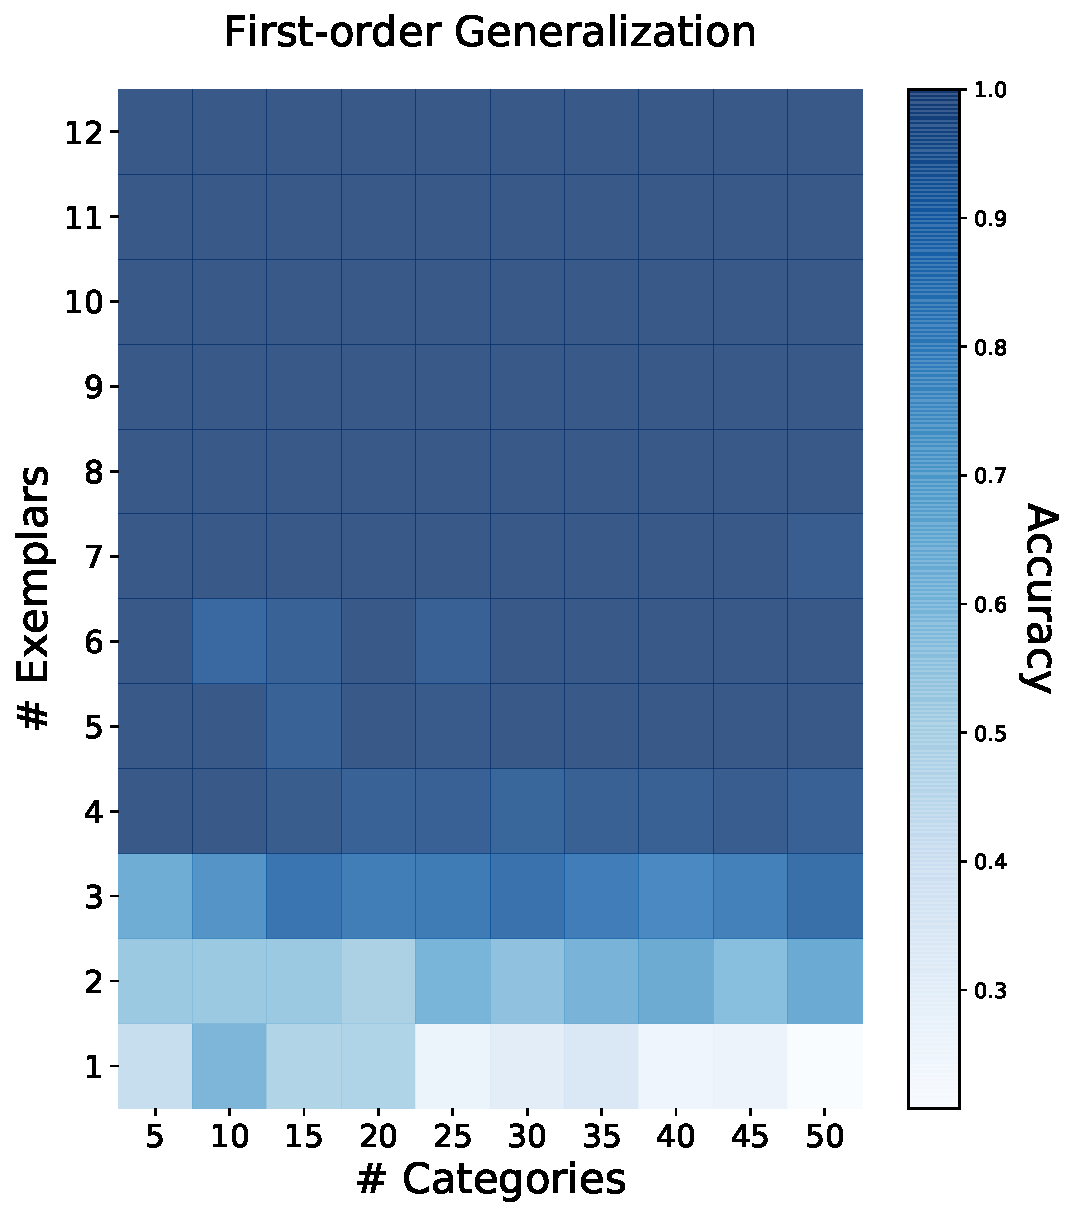
\includegraphics[width=0.98\textwidth]{figures/mlp_1order_accuracy.pdf}
                    \end{center}
                \end{subfigure}
                % subfigure (b)
                \begin{subfigure}[b]{0.48\textwidth}
                    \begin{center}
                        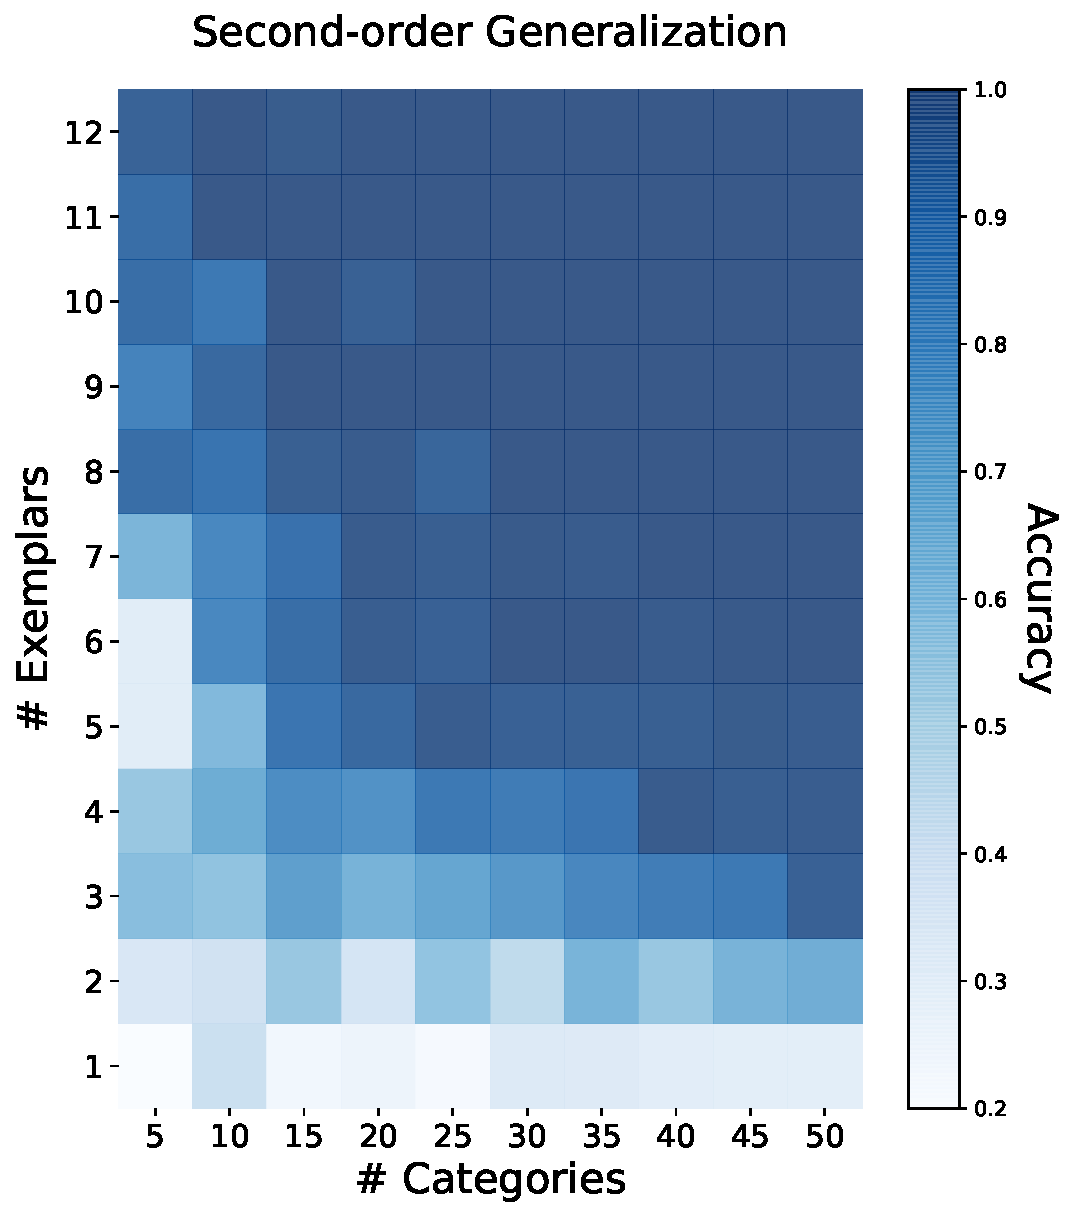
\includegraphics[width=0.98\textwidth]{figures/mlp_2order_accuracy.pdf}
                    \end{center}
                \end{subfigure}
            \end{center}
            \caption{MLP}
            \label{fig:mlp_results}
        \end{subfigure}
        % cnn results
        \begin{subfigure}[b]{0.47\textwidth}
            \begin{center}
                % subfigure (a)
                \begin{subfigure}[b]{0.48\textwidth}
                    \begin{center}
                        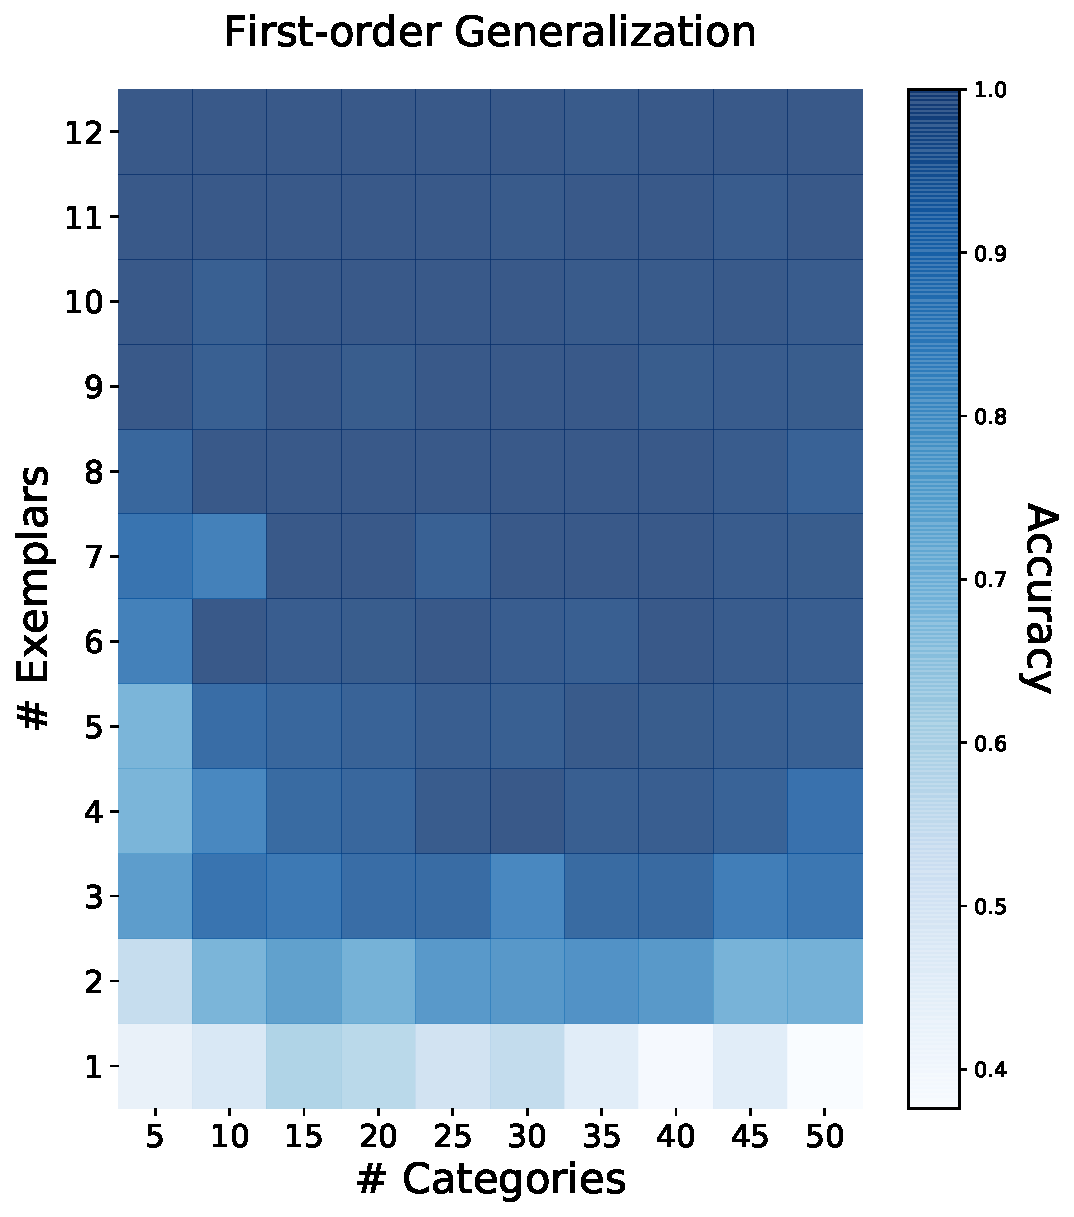
\includegraphics[width=\textwidth]{figures/cnn_1order_accuracy.pdf}
                    \end{center}
                \end{subfigure}
                % subfigure (b)
                \begin{subfigure}[b]{0.48\textwidth}
                    \begin{center}
                        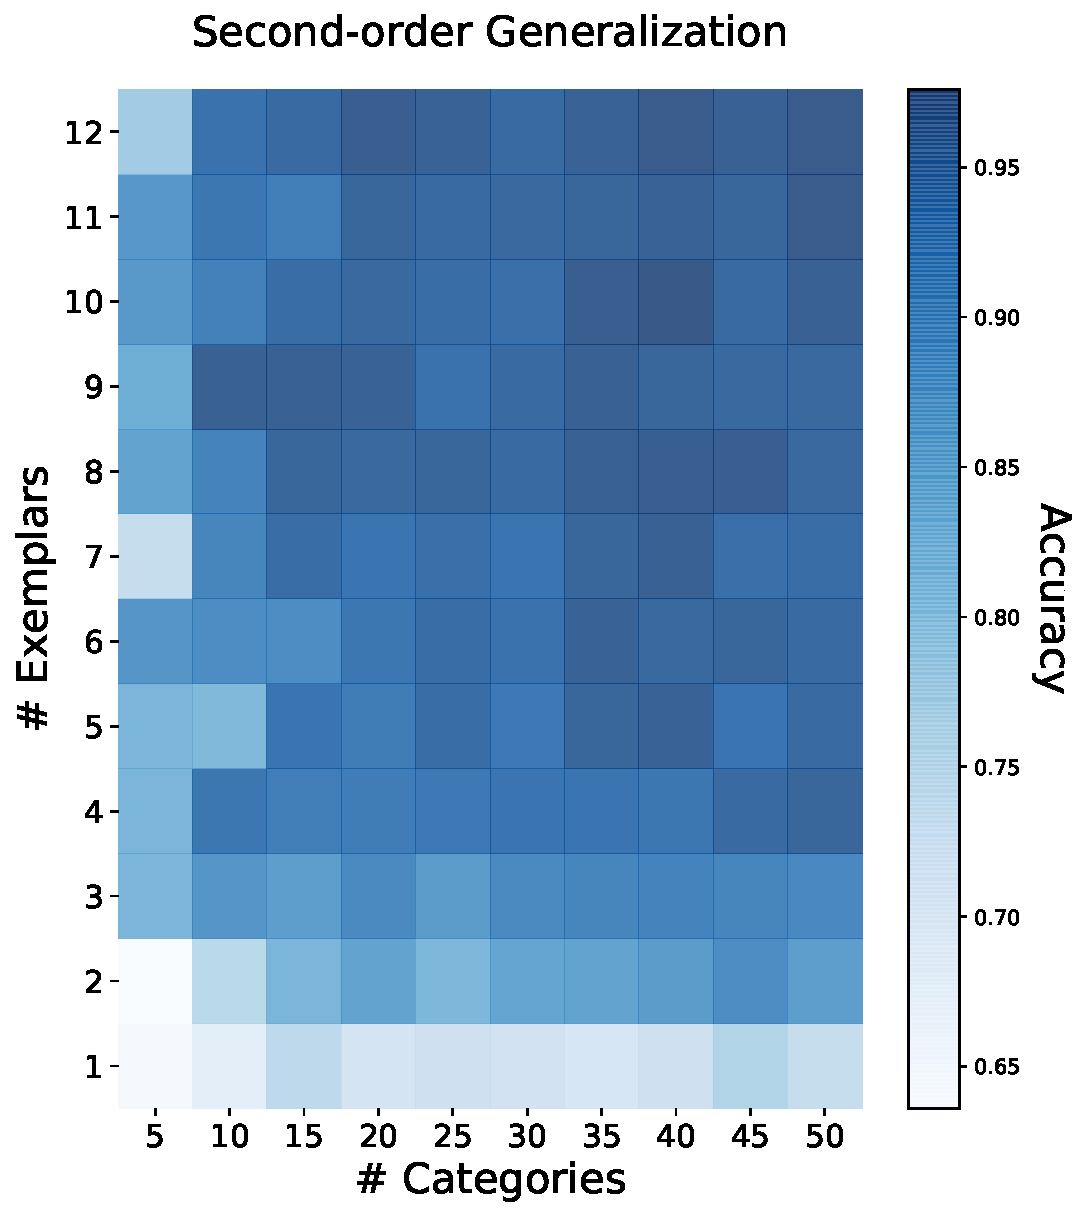
\includegraphics[width=\textwidth]{figures/cnn_2order_accuracy.pdf}
                    \end{center}
                \end{subfigure}
            \end{center}
            \caption{CNN}
            \label{fig:cnn_results}
        \end{subfigure}
    \end{center}
    \caption{First- and second-order generalization results for the simple MLP
    and CNN models. For each \{\textit{\# categories}, \textit{\# exemplars}\}
    pair, the average result from 5 trials is shown.}
    \label{fig:generalization_results}
\end{figure*}
\section{Multilayer Perceptron Trained on Synthetic Objects}
\label{sec:simple_mlp}

In our first experiment, we encode the categorical stimulus information of our
synthetic objects as abstract patterns, representing the shape, color and
texture features each as independent 20-bit vectors. The overall stimulus thus
has 60 bits. The categories of each feature are assigned their bit-vector representations
randomly at the beginning of the experiment. We train a multilayer perceptron (MLP)
with one hidden layer of 30 ReLU units to classify the shape of the presented
stimulus. The number of units in the softmax layer varies with the
\textit{\# categories} dataset parameter. To mimick the control group of
\cite{Smith2002}, we initialized our MLP model randomly and evaluated
second-order generalization results prior to training. The model selected by
shape X\%, color X\% and texture X\% We then trained our model with various
dataset sizes. Results for each the first- and second-order generalizations,
averaged over 10 training runs, are shown in Fig. \ref{fig:mlp_gen_results}.
TODO: discuss results.

To analyze the parametric dependency of network biases on the presented
stimuli, we perform a series of tests using a network trained with 50 categories
and 15 exemplars. For the first test, we probe the shape bias of our MLP by
varying the shape distance between two presented stimuli and recording the resulting
network similarity score at each input pair, using cosine similarity at the
hidden layer. Distance in shape space is quantified as the fraction of bits that
differ along the 20-bit space denoted to shape. Similar tests are also performed
for the color and texture features. Results are shown in Fig.
\ref{fig:mlp_parametric}. TODO: discuss results.

\begin{figure}[h!]
    \begin{center}
        \begin{subfigure}[b]{0.235\textwidth}
            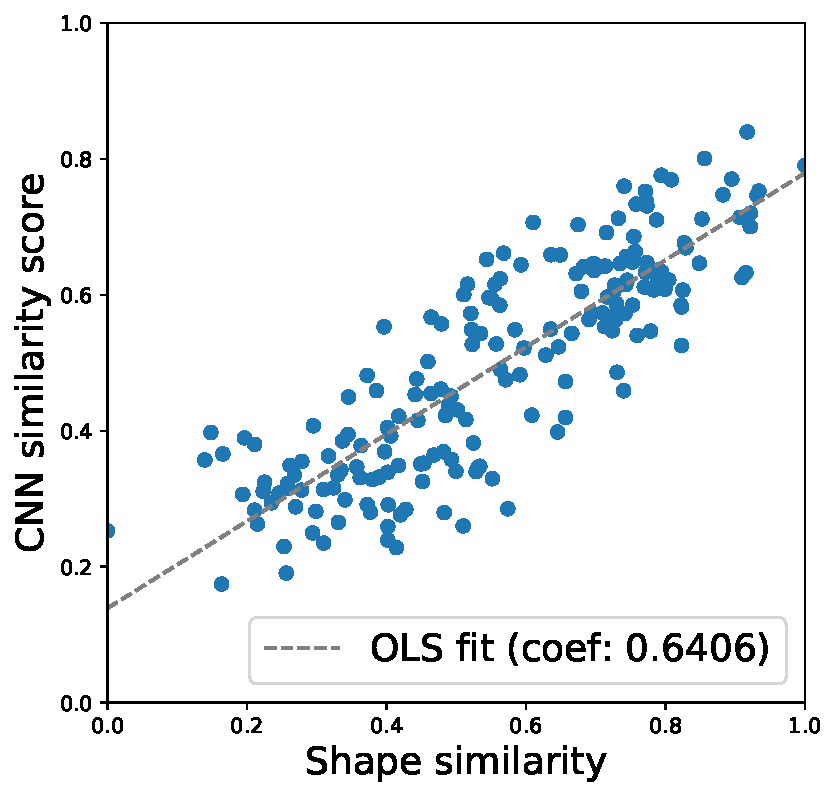
\includegraphics[width=\linewidth]
            {figures/vgg_shape_parametric_others_constant.pdf}
            \caption{Shape}
        \end{subfigure}
        \begin{subfigure}[b]{0.235\textwidth}
            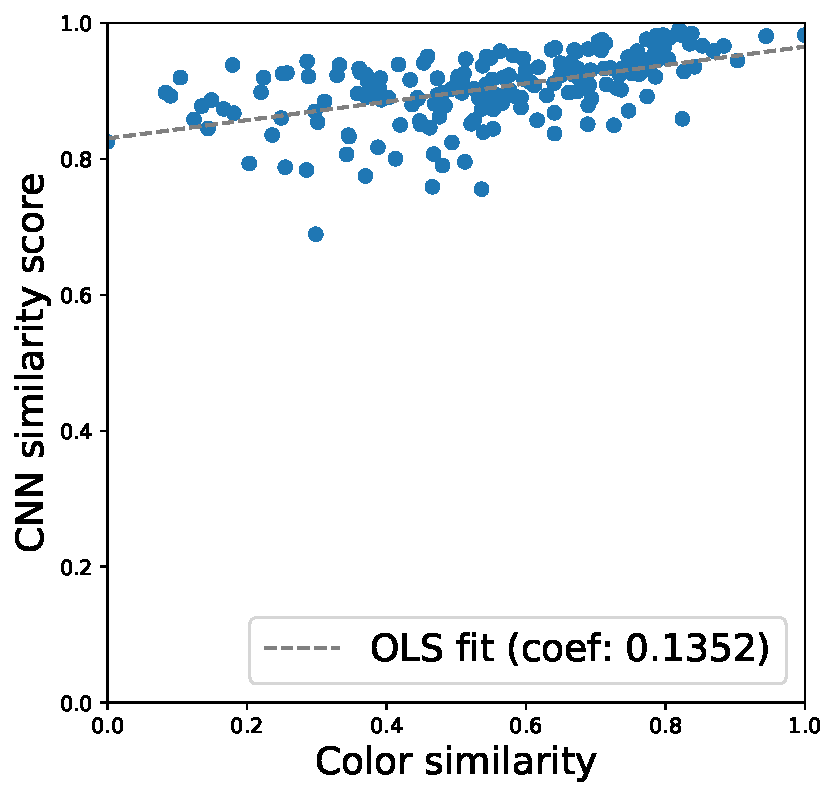
\includegraphics[width=\linewidth]
            {figures/vgg_color_parametric_others_constant.pdf}
            \caption{Color}
        \end{subfigure}
    \end{center}
    \caption{MLP parametric shape and color biases. TODO: put correct result
    plots here.}
    \label{fig:mlp_parametric}
\end{figure}
\section{Convolutional Network Trained on Synthetic Objects}
\label{sec:simple_cnn}

% cnn generalization results
\begin{figure*}[t]
    \begin{center}
        % subfigure (a)
        \begin{subfigure}[b]{0.48\textwidth}
            \begin{center}
                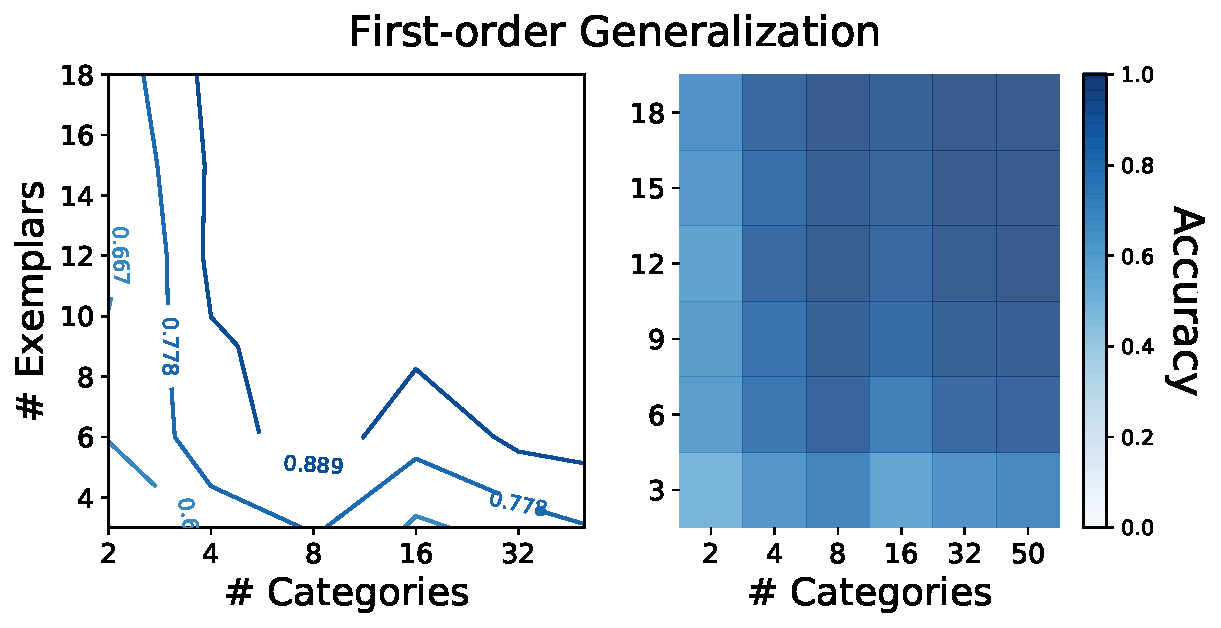
\includegraphics[width=0.98\textwidth]
                {figures/cnn_o1_acc.pdf}
            \end{center}
        \end{subfigure}
        % subfigure (b)
        \begin{subfigure}[b]{0.48\textwidth}
            \begin{center}
                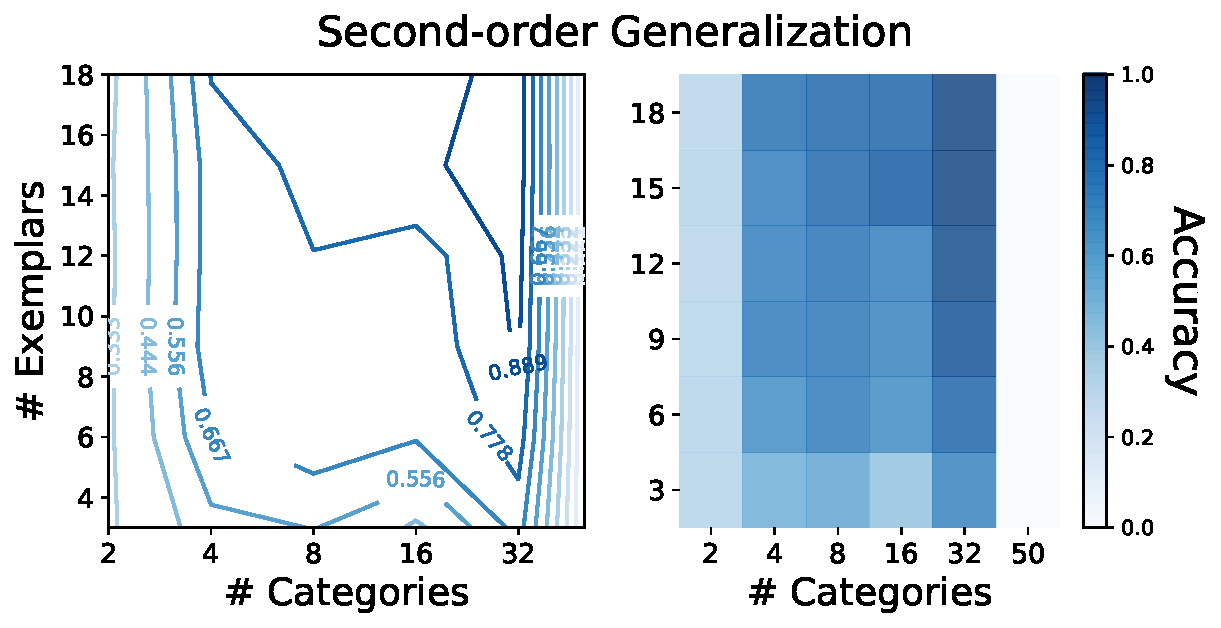
\includegraphics[width=0.98\textwidth]
                {figures/cnn_o2_acc.pdf}
            \end{center}
        \end{subfigure}
    \end{center}
    \caption{CNN generalization results for various training set sizes. Results
    show the average from 10 trials.}
    \label{fig:cnn_gen_results}
\end{figure*}

Our first experiment uses a very simple data form. However, neural network
architectures can achieve success with highly complex data, including natural
images, language and audio. In a successive experiment, ask whether similar
generalization results can be achieved using object stimuli encoded as RGB
images. To do so, we construct an image dataset consisting of artifical 2D
objects. Each object is a 2D shape of a specified color placed over white background.
Objects are initially centered, however, a random shift is applied to every sample.
Texture is represented in a fourth dimension, independent of RGB space. The motivation for this design choice
is as follows. In the experiments of \cite{Smith2002}, children physically touch
each object that they are presented in addition to observing it visually. Although the
presence of materials like plastic and styrofoam may be visually subtle compared
to color and shape, these materials become much more detectable when sensed by hand.
Since visual and touch signals are received along separate pathways, it makes
sense to provide these signals along independent axes to a computational model.

Object shapes are determined by randomly generating sets of points around the 2D
image window, and colors are generated to span the RGB vector space with even
separation. We use black \& white textures from the Brodatz database \citep{Brodatz1966}
for our texture categories. Some examples of our objects are shown in Fig.
\ref{fig:generated_images}. We train a convolutional neural network (CNN)
consisting of 2 convolution layers with 5 filters, each followed by a max pooling
layer. The last pooling layer is followed by a fully-connected layer of 25 ReLU
units, and the softmax layer again varies in size according to the number of
categories in the dataset. The initial second-order generalization results for a
random network are as follows: shape 0.39, color 0.41 and texture 0.20.
Results for networks trained on various dataset sizes are shown in Fig. \ref{fig:cnn_gen_results}.

We next analyze the parametric relationship between our CNN biases and the feature
values of presented stimuli similarly to our MLP. For our image objects,
distance in shape space is quantified as the Modified Hausdorff Distance
\citep{Dubuisson1994} between the shape pair. In color space, distance is
quantified using the cosine similarity of the RGB vector pair. The parametric
bias results are shown in Fig. \ref{fig:cnn_parametric}.

\begin{figure}[t!]
    \begin{center}
        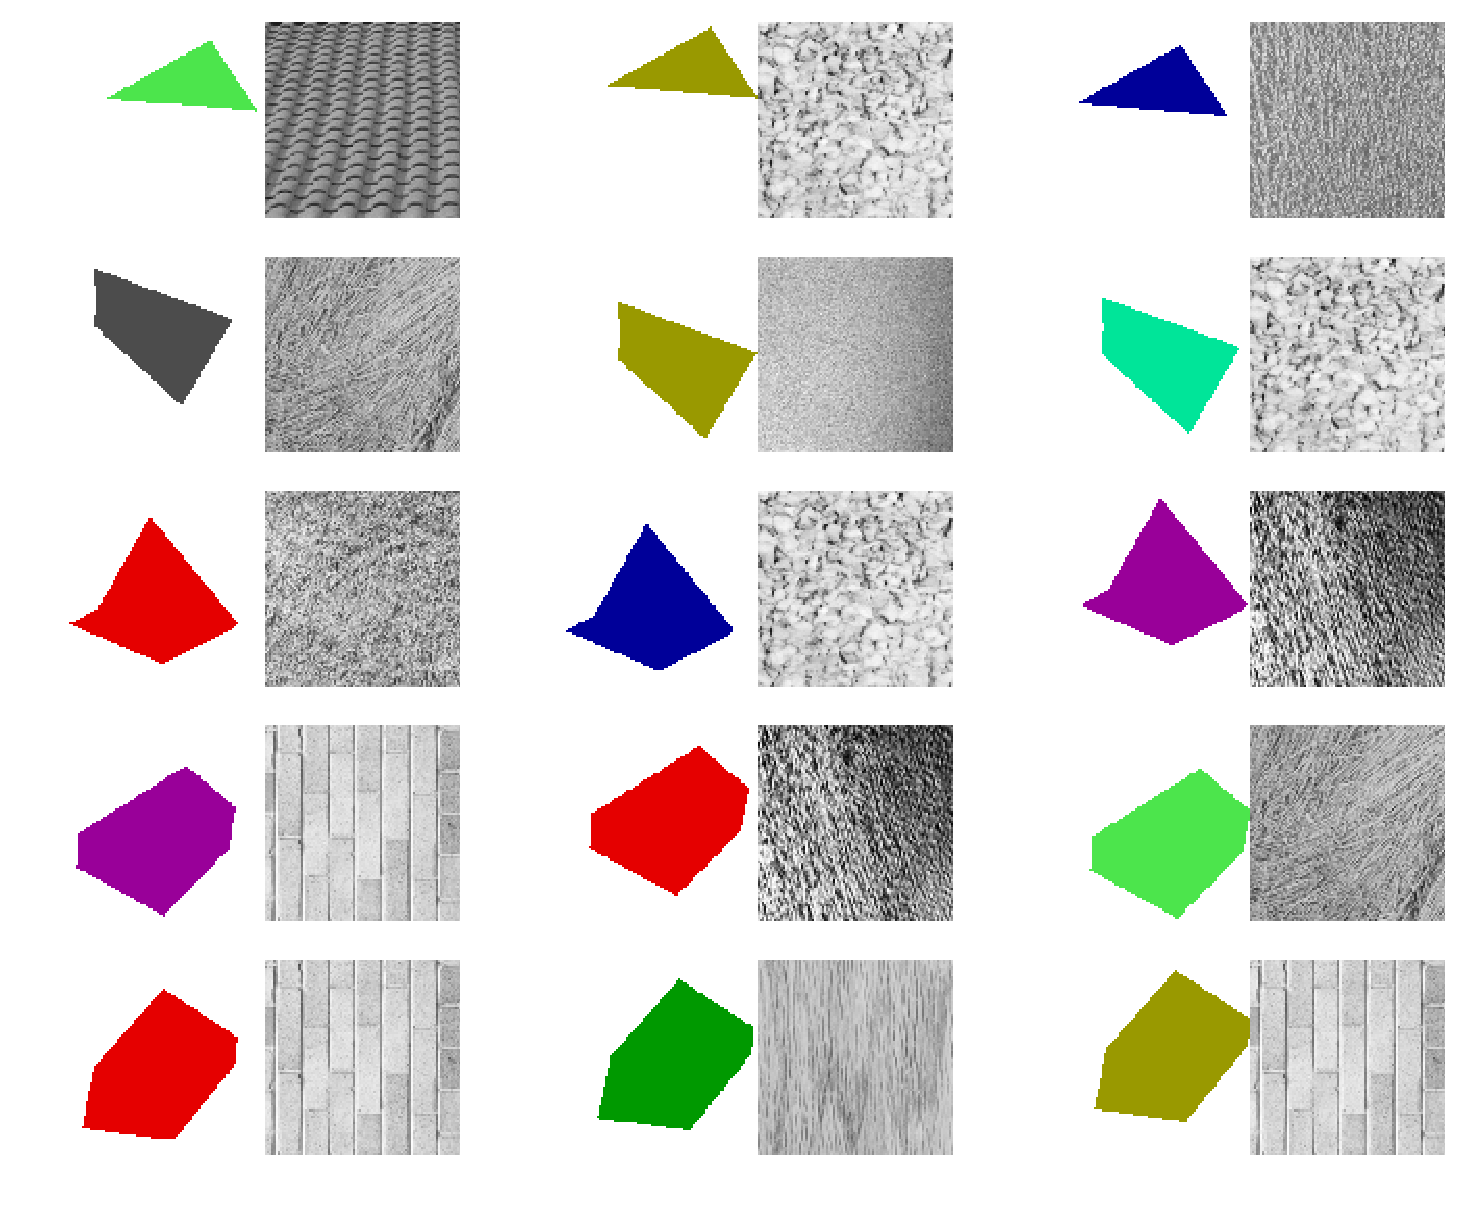
\includegraphics[width=0.48\textwidth]{figures/generated_images.pdf}
    \end{center}
    \caption{Computer-generated images of 2D objects with
    different shape, color and texture features.}
    \label{fig:generated_images}
\end{figure}

\begin{figure}[h!]
    \begin{center}
        \begin{subfigure}[b]{0.235\textwidth}
            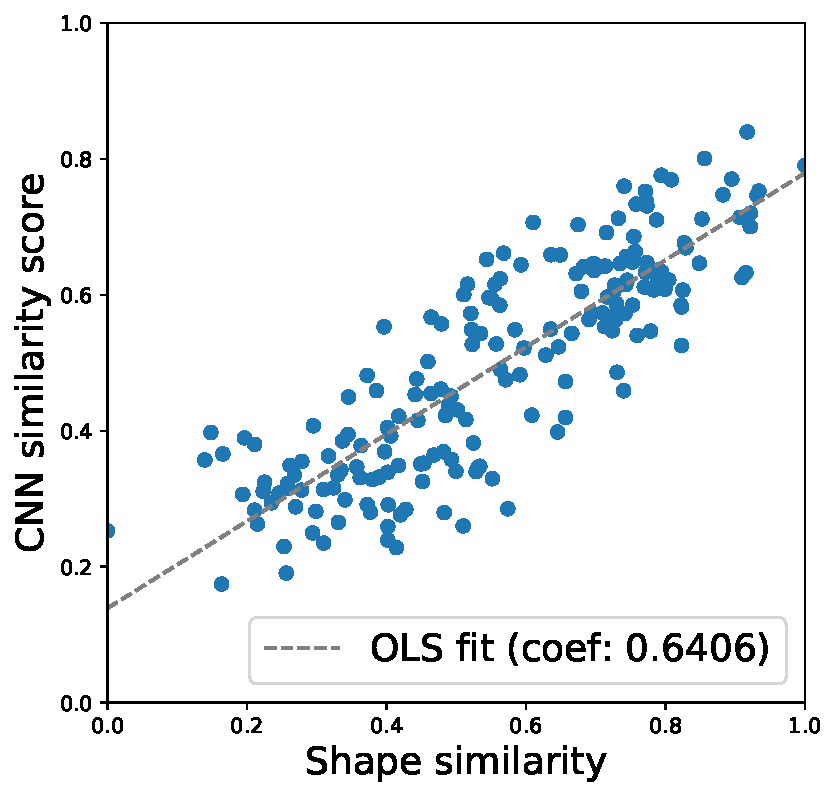
\includegraphics[width=\linewidth]
            {figures/vgg_shape_parametric_others_constant.pdf}
            \caption{Shape}
        \end{subfigure}
        \begin{subfigure}[b]{0.235\textwidth}
            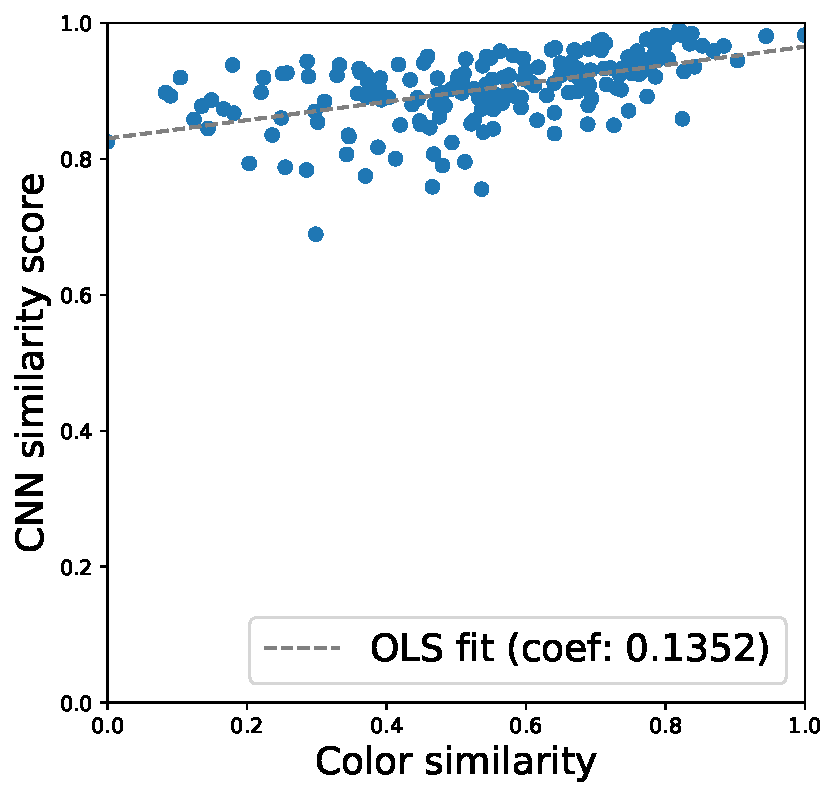
\includegraphics[width=\linewidth]
            {figures/vgg_color_parametric_others_constant.pdf}
            \caption{Color}
        \end{subfigure}
    \end{center}
    \caption{CNN parametric shape and color biases. TODO: put correct result
    plots here.}
    \label{fig:cnn_parametric}
\end{figure}

% \begin{figure}[h!]
%     \begin{center}
%         % shape 1
%         \begin{subfigure}[b]{0.15\textwidth}
%             \begin{center}
%                 \begin{subfigure}[b]{0.9\textwidth}
%                     \includegraphics[width=\linewidth]
%                     {figures/artist_objects/fake1_carpet_red.jpg}
%                 \end{subfigure}
%                 \begin{subfigure}[b]{0.9\textwidth}
%                     \includegraphics[width=\linewidth]
%                     {figures/artist_objects/fake1_sponge_yellow.jpg}
%                 \end{subfigure}
%             \end{center}
%         \end{subfigure}
%         % % shape 2
%         \begin{subfigure}[b]{0.15\textwidth}
%             \begin{center}
%                 \begin{subfigure}[b]{0.9\textwidth}
%                     \includegraphics[width=\linewidth]
%                     {figures/artist_objects/fake5_wood_pink.jpg}
%                 \end{subfigure}
%                 \begin{subfigure}[b]{0.9\textwidth}
%                     \includegraphics[width=\linewidth]
%                     {figures/artist_objects/fake5_carpet_purple.jpg}
%                 \end{subfigure}
%             \end{center}
%         \end{subfigure}
%         \begin{subfigure}[b]{0.15\textwidth}
%             \begin{center}
%                 \begin{subfigure}[b]{0.9\textwidth}
%                     \includegraphics[width=\linewidth]
%                     {figures/artist_objects/fake4_sponge_orange.jpg}
%                 \end{subfigure}
%                 \begin{subfigure}[b]{0.9\textwidth}
%                     \includegraphics[width=\linewidth]
%                     {figures/artist_objects/fake4_wood_green.jpg}
%                 \end{subfigure}
%             \end{center}
%         \end{subfigure}
%     \end{center}
%     \caption{Artist-designed images of 3D objects with different shape, color
%     and texture features.}
%     \label{fig:artist_images}
% \end{figure}

% \subsection{Layer-wise Biases}
% The first step of our analysis is to evaluate the shape, color and texture biases of VGG-16
% at each of its layers, in order to get a picture of how these biases develops along the
% higherarchy of the model's internal representation. In order to probe the model, we make
% use of two unique image datasets with stimuli that mimic \cite{Smith2002}.

% {\bf1. Artist-generated object dataset}: These images were generated by an artist in Adobe
% Photoshop. See Fig. \ref{fig:artist_images}.

% {\bf2. CogPsyc object dataset}: These images were provided by cognitive psychologist Linda
% Smith, and they were used in the experiments of \cite{Ritter2017}. See Fig.
% \ref{fig:cogpsyc_images}.

% \begin{figure*}[h]
%     \begin{center}
%         \begin{subfigure}[b]{0.4\textwidth}
%             \begin{center}
%                 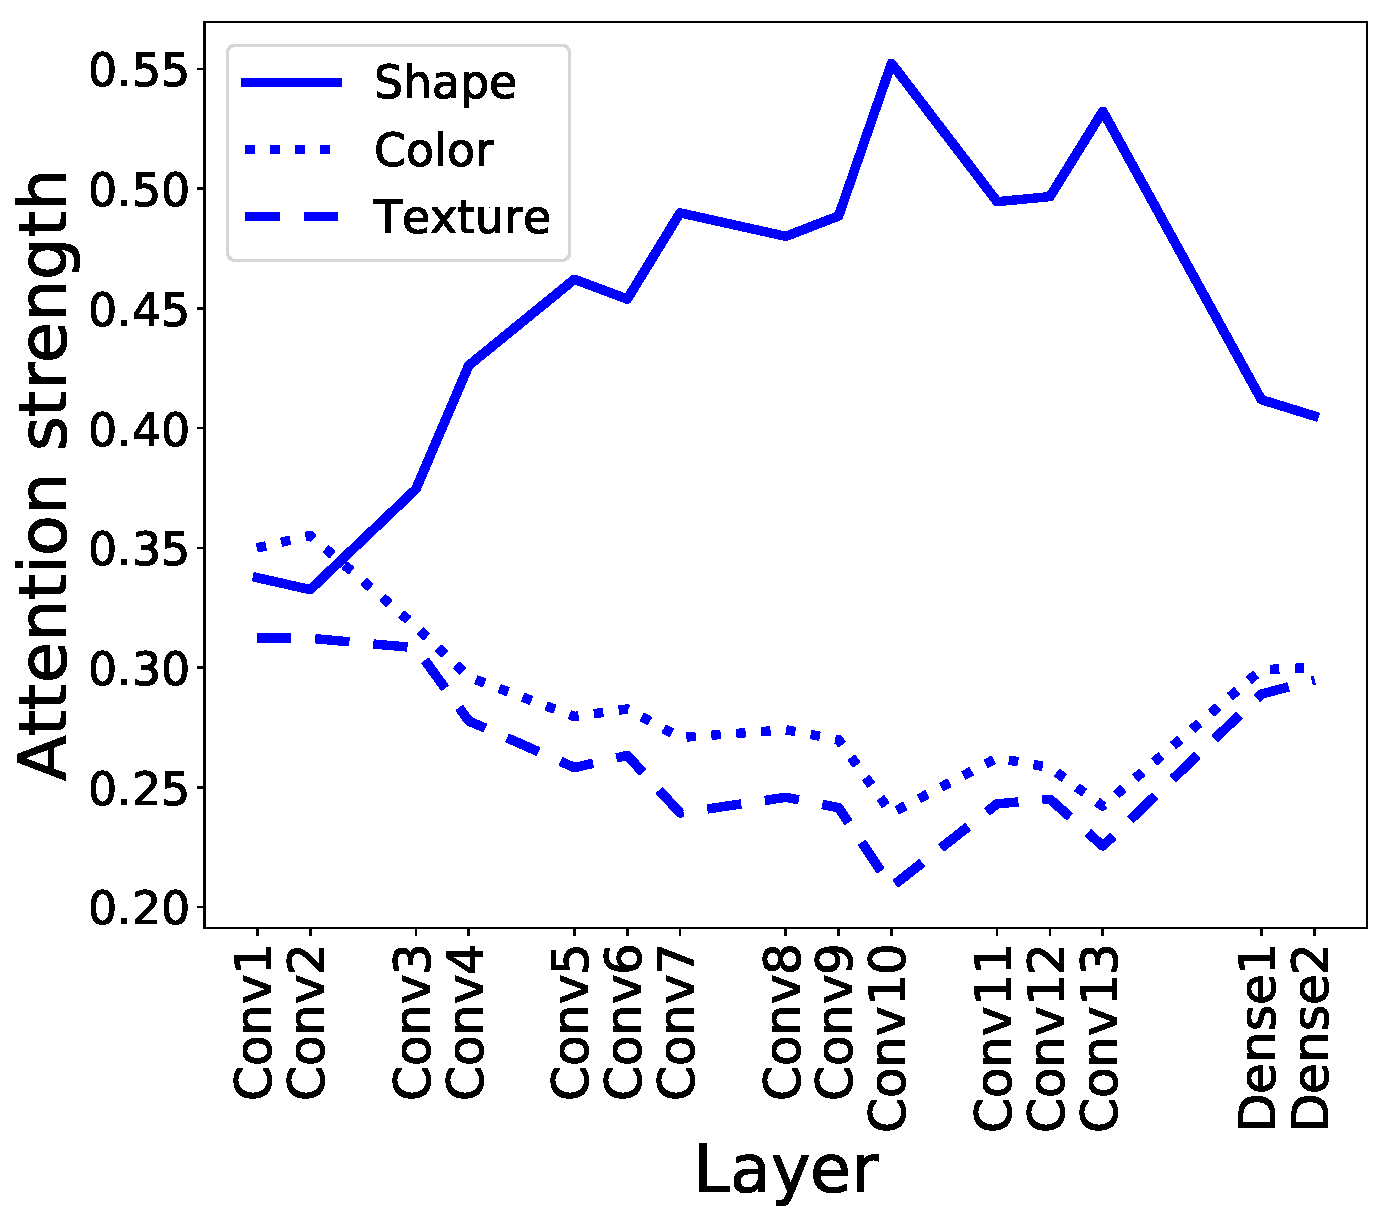
\includegraphics[width=\textwidth]{figures/vgg_layer_biases.pdf}
%             \end{center}
%             \caption{Artist-generated images}
%             \label{fig:biases_artist}
%         \end{subfigure}
%         \begin{subfigure}[b]{0.4\textwidth}
%             \caption{CogPsyc images (TODO)}
%         \end{subfigure}
%         \caption{VGG-16 layer-wise biases on two image datasets. Attention strength refers to
%         the network's similarity score between the target objectand objects that match in
%         either shape, color or texture.}
%     \end{center}
%     \label{fig:layerwise_biases}
% \end{figure*}

% \begin{figure}[h!]
%     \begin{center}
%         \begin{subfigure}[b]{0.235\textwidth}
%             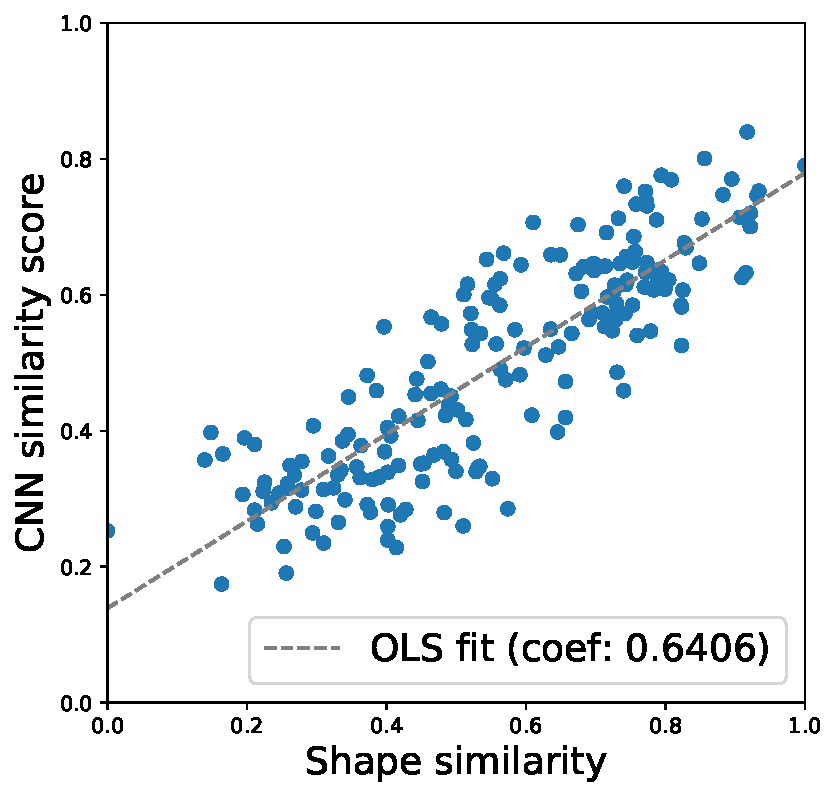
\includegraphics[width=\linewidth]{figures/vgg_shape_parametric_others_constant.pdf}
%             \caption{Shape}
%         \end{subfigure}
%         \begin{subfigure}[b]{0.235\textwidth}
%             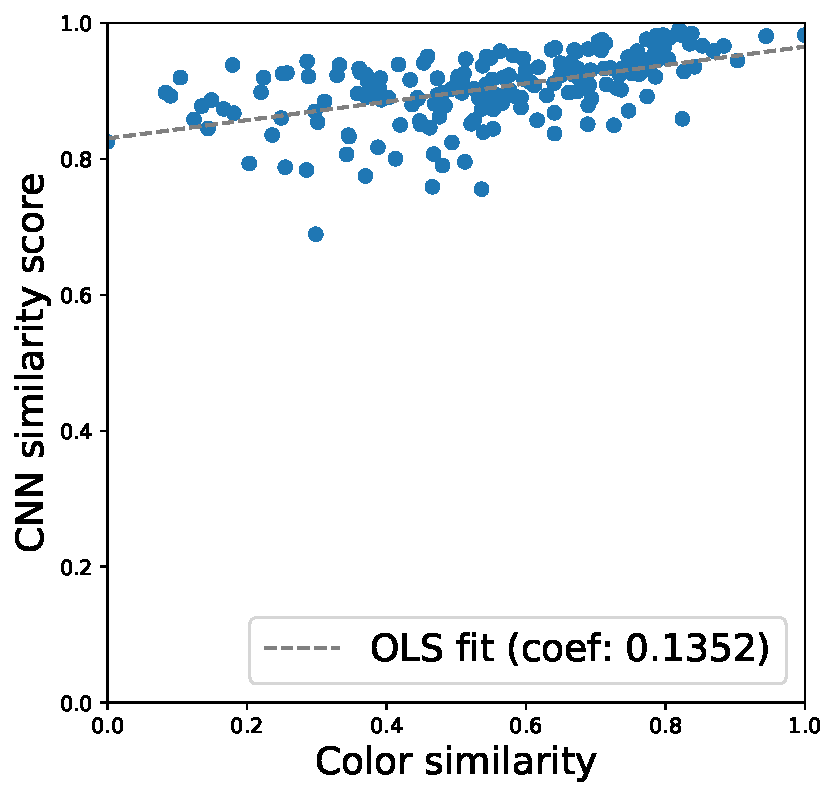
\includegraphics[width=\linewidth]{figures/vgg_color_parametric_others_constant.pdf}
%             \caption{Color}
%         \end{subfigure}
%     \end{center}
%     \caption{VGG-16 parametric shape and color biases w/ other features constant.}
%     \label{fig:parametric_others_constant}
% \end{figure}

% \begin{figure}[h!]
%     \begin{center}
%         \begin{subfigure}[b]{0.235\textwidth}
%             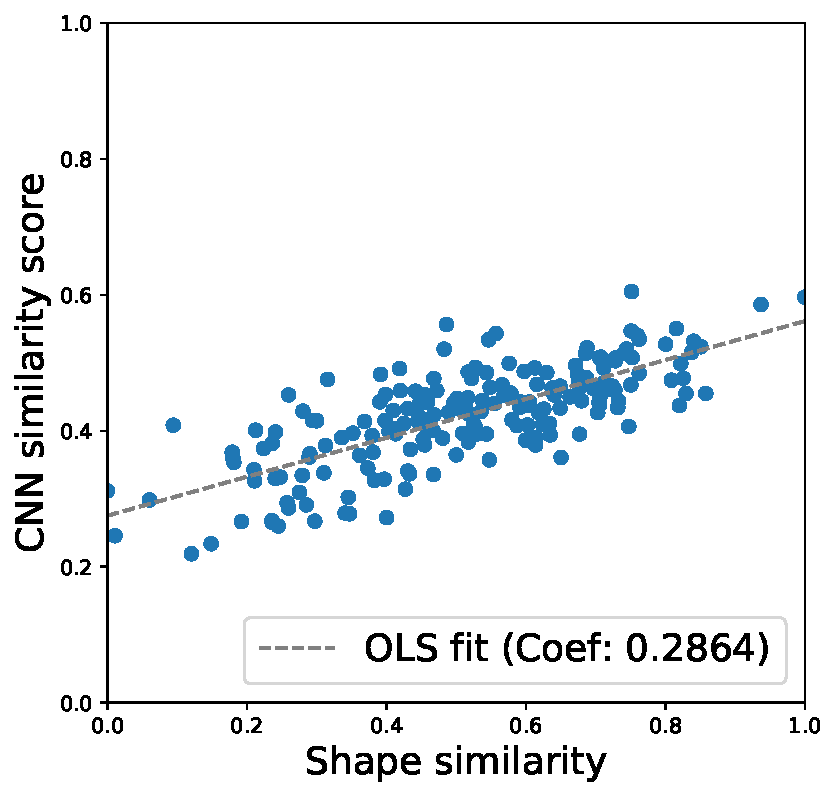
\includegraphics[width=\linewidth]{figures/vgg_shape_parametric.pdf}
%             \caption{Shape}
%         \end{subfigure}
%         \begin{subfigure}[b]{0.235\textwidth}
%             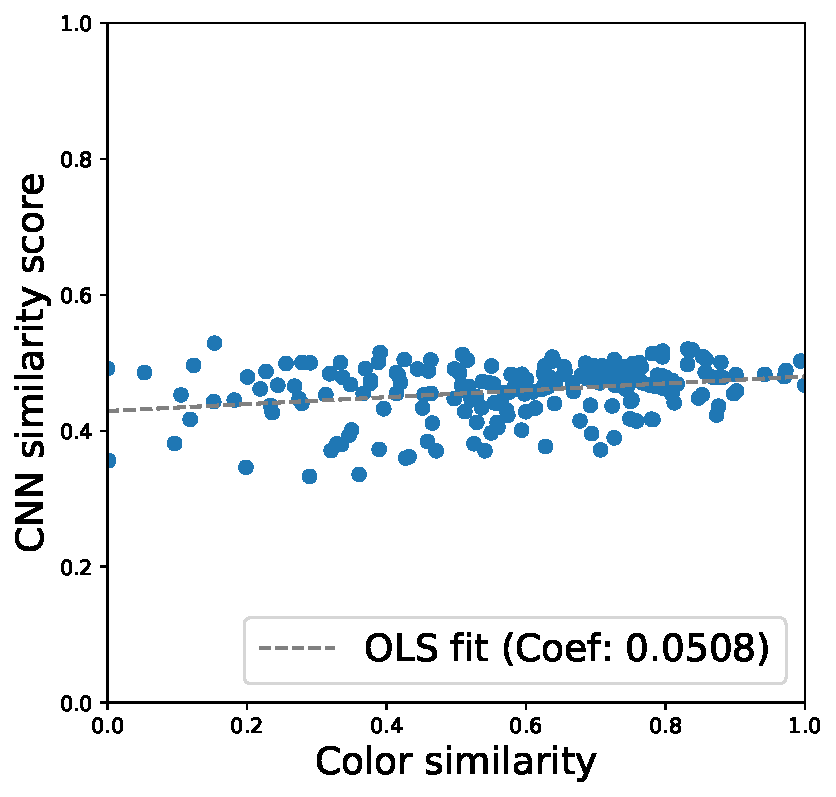
\includegraphics[width=\linewidth]{figures/vgg_color_parametric.pdf}
%             \caption{Color}
%         \end{subfigure}
%     \end{center}
%     \caption{VGG-16 parametric shape and color biases w/ other features varying.}
%     \label{fig:parametric_others_varying}
% \end{figure}
\section{Predicting the Onset of Vocabulary Acceleration}
\section{Discussion}
Our experiments in this paper confirm that neural networks are capabable
of developing the shape bias from as few as three examples of each object category.
The development of this bias is known to improve the rate of word learning in
human children, a phenomenon that is mirrored in our networks. One implication
of this finding is that it may be possible to train
large-scale image recognition models more efficiently after initializing these
models with shape bias training. In future work, we hope to investigate this
hypothesis with ImageNet CNN models using an initialization framework designed
after the experiments in this paper.

Philosophers of science have discussed the importance of prior background knowledge
for centuries \citep{Tenenbaum2011}. When the data provided to a learner is scarce, these
priors help fill in the gap by constraining the space of models that the learner
must consider. A new theory suggests that this phenomenon can be
quantified from the perspective of information theory \citep{Mattingly2017}.
Authors of the report show that, given an appropriate choice of prior over model
space, a learner can maximize the amount of information extracted from limited
data. They formalize this claim using the mutual information between the
observed data and the parameters of the model. This measure quantifies the amount
of information that can be learned about the model by measuring the data, or
equivalently, the information about the data that can be encoded in the model.
The information theory framework explains why structured model priors are
helpful when data is scarce. The case of structured Bayesian priors is contrasted
against that of a flat prior (i.e. no prior), with the former showing clear
advantages.

TODO: final paragraph. What is left to discuss?
\section{Acknowledgements}

This research was supported by a Henry M. McCracken fellowship and NYU
start-up faculty funding (?). We thank Subhankar Ghosh for useful code and
preliminary experiment ideas.

\bibliographystyle{apacite}

\setlength{\bibleftmargin}{.125in}
\setlength{\bibindent}{-\bibleftmargin}

\bibliography{citations}


\end{document}
